\chapter{Umsetzung der interaktiven Benutzeroberfläche}
\label{chapter:umsetzung-der-interaktiven-benutzeroberfläche}

TODO:


\begin{figure}[!ht]
    \centering
    \begin{tikzpicture}
        \node [inner sep=0pt,,outer sep=0pt,clip,rounded corners=0.15cm] (image) at (0,0) {
            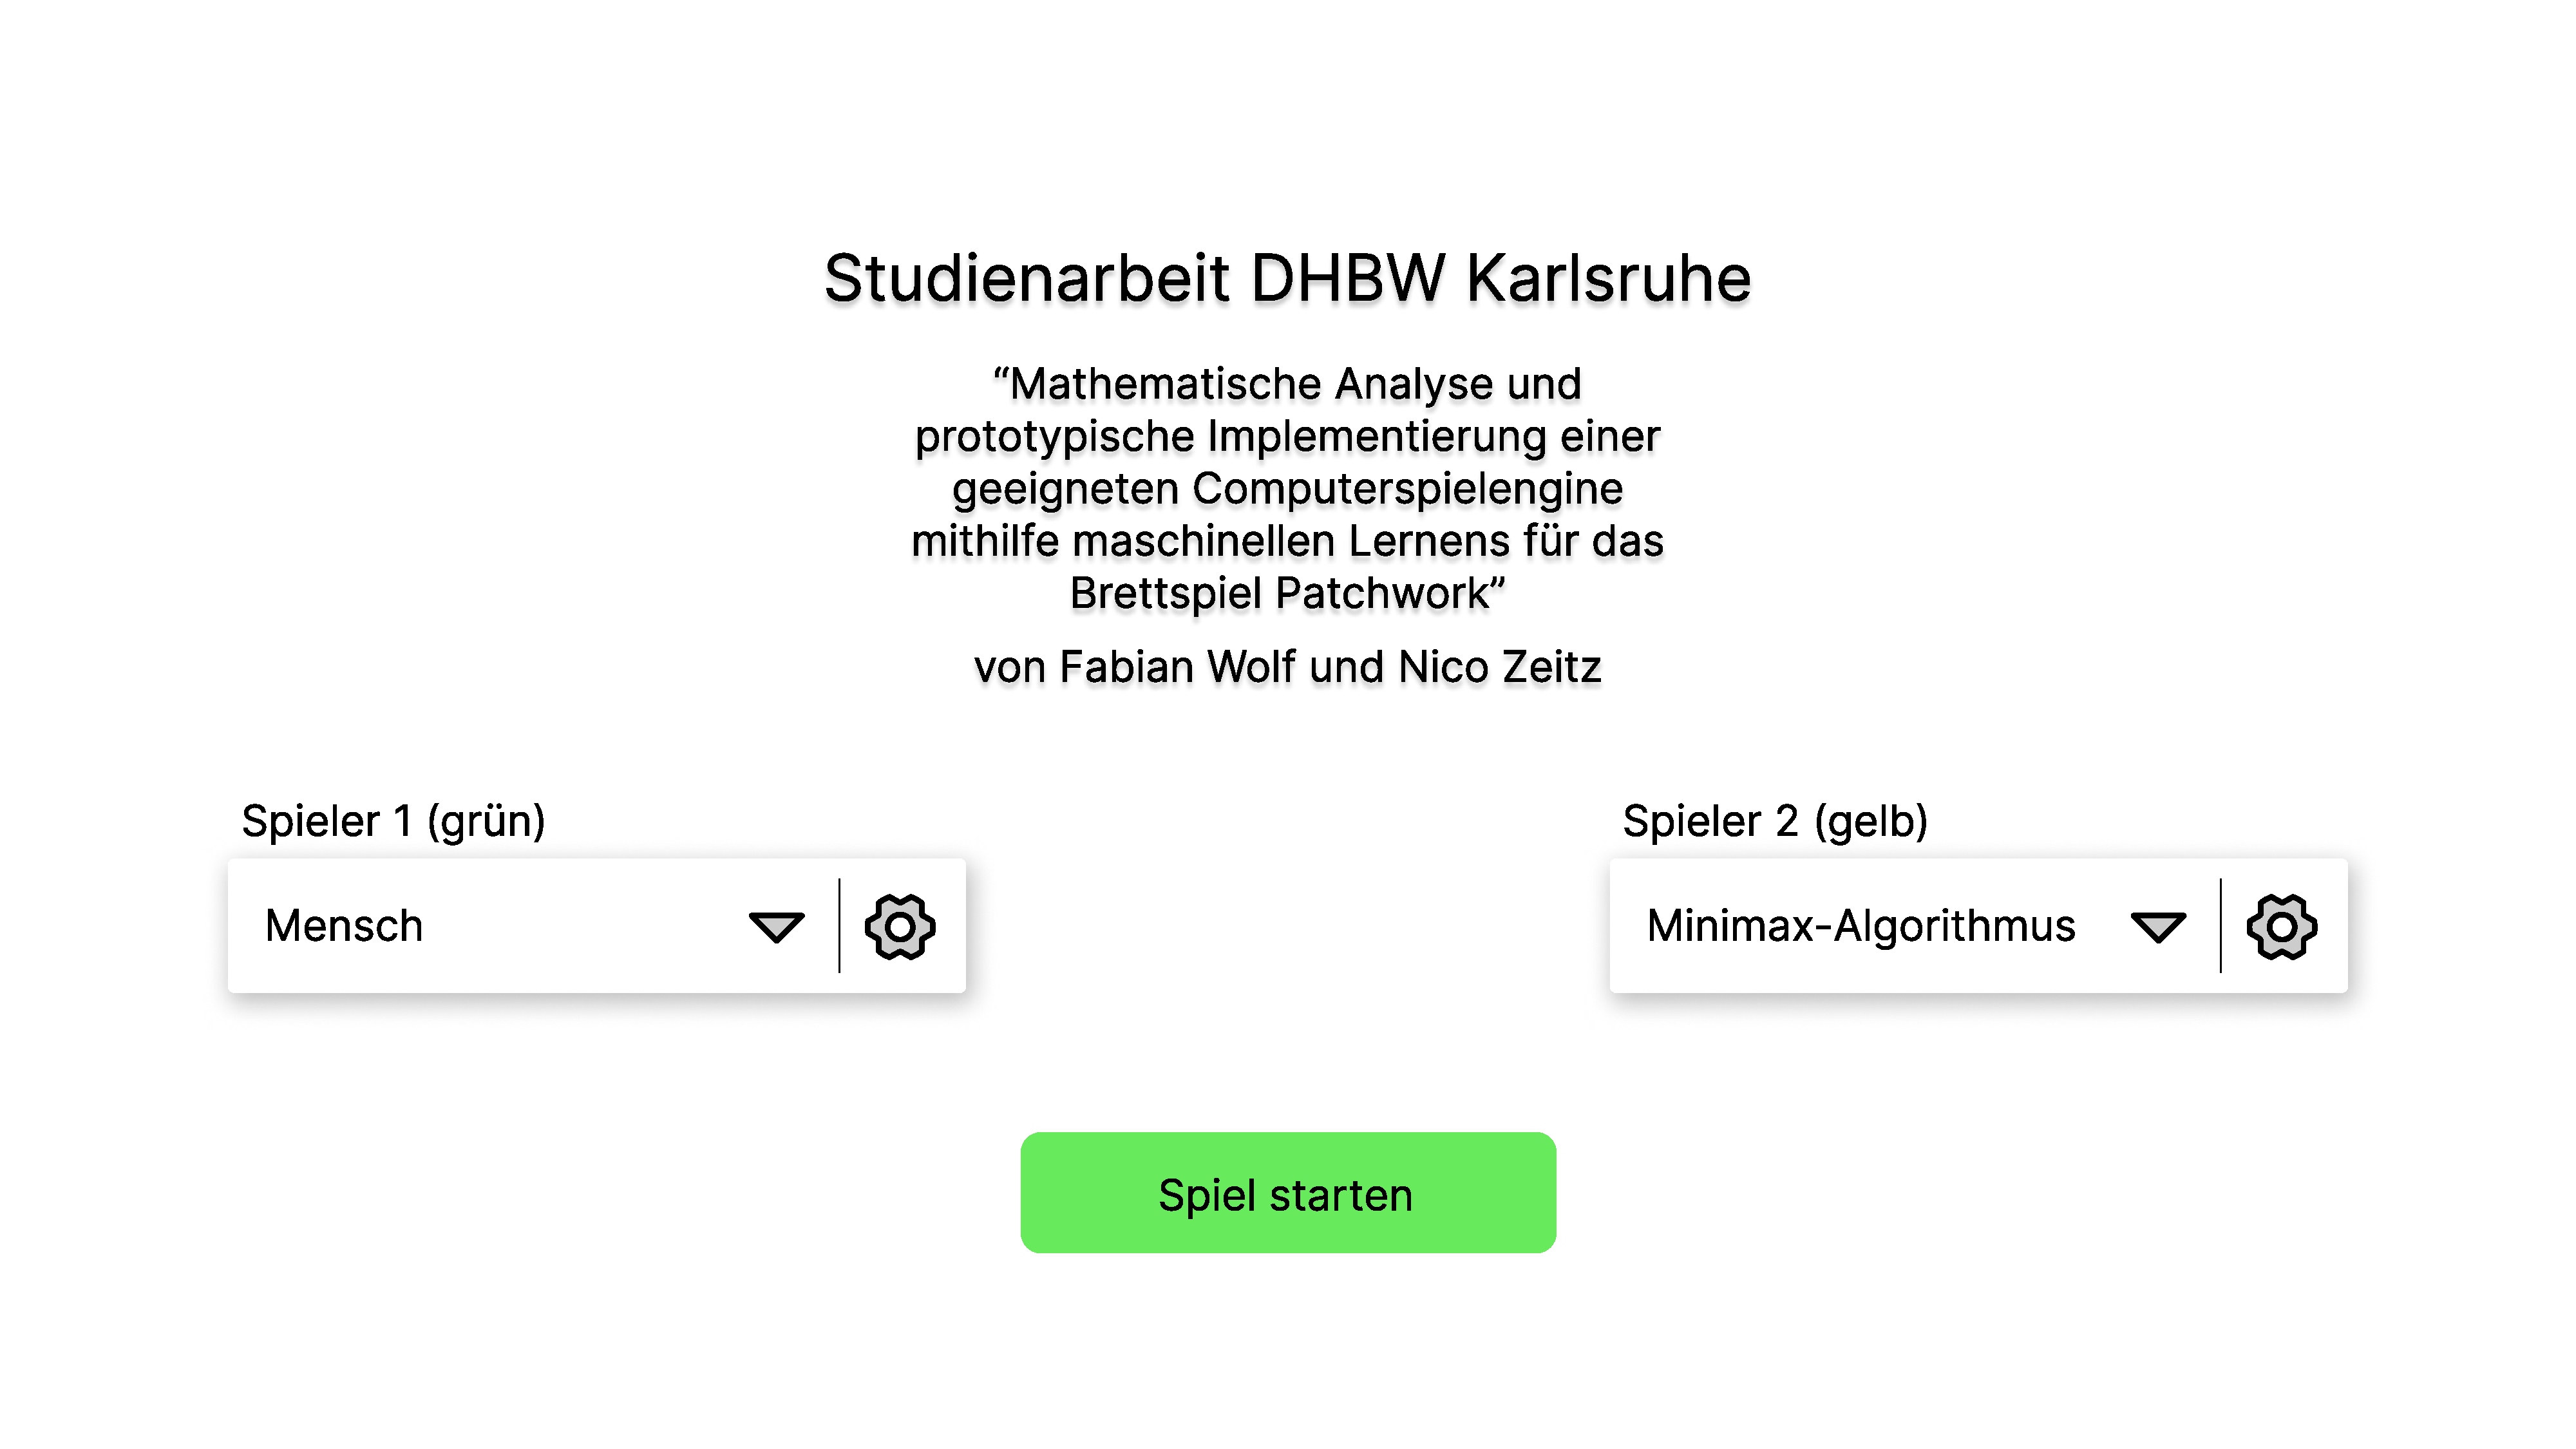
\includegraphics[width=\textwidth]{res/pictures/desig_main_ui.pdf}};
        \drawshadow{image}
    \end{tikzpicture}
    \caption{Designentwurf vom Hauptmenü des Computerspiel}
    \label{fig:design-main-ui}
\end{figure}

\begin{figure}[!ht]
    \centering
    \begin{tikzpicture}
        \node [inner sep=0pt,,outer sep=0pt,clip,rounded corners=0.15cm] (image) at (0,0) {
            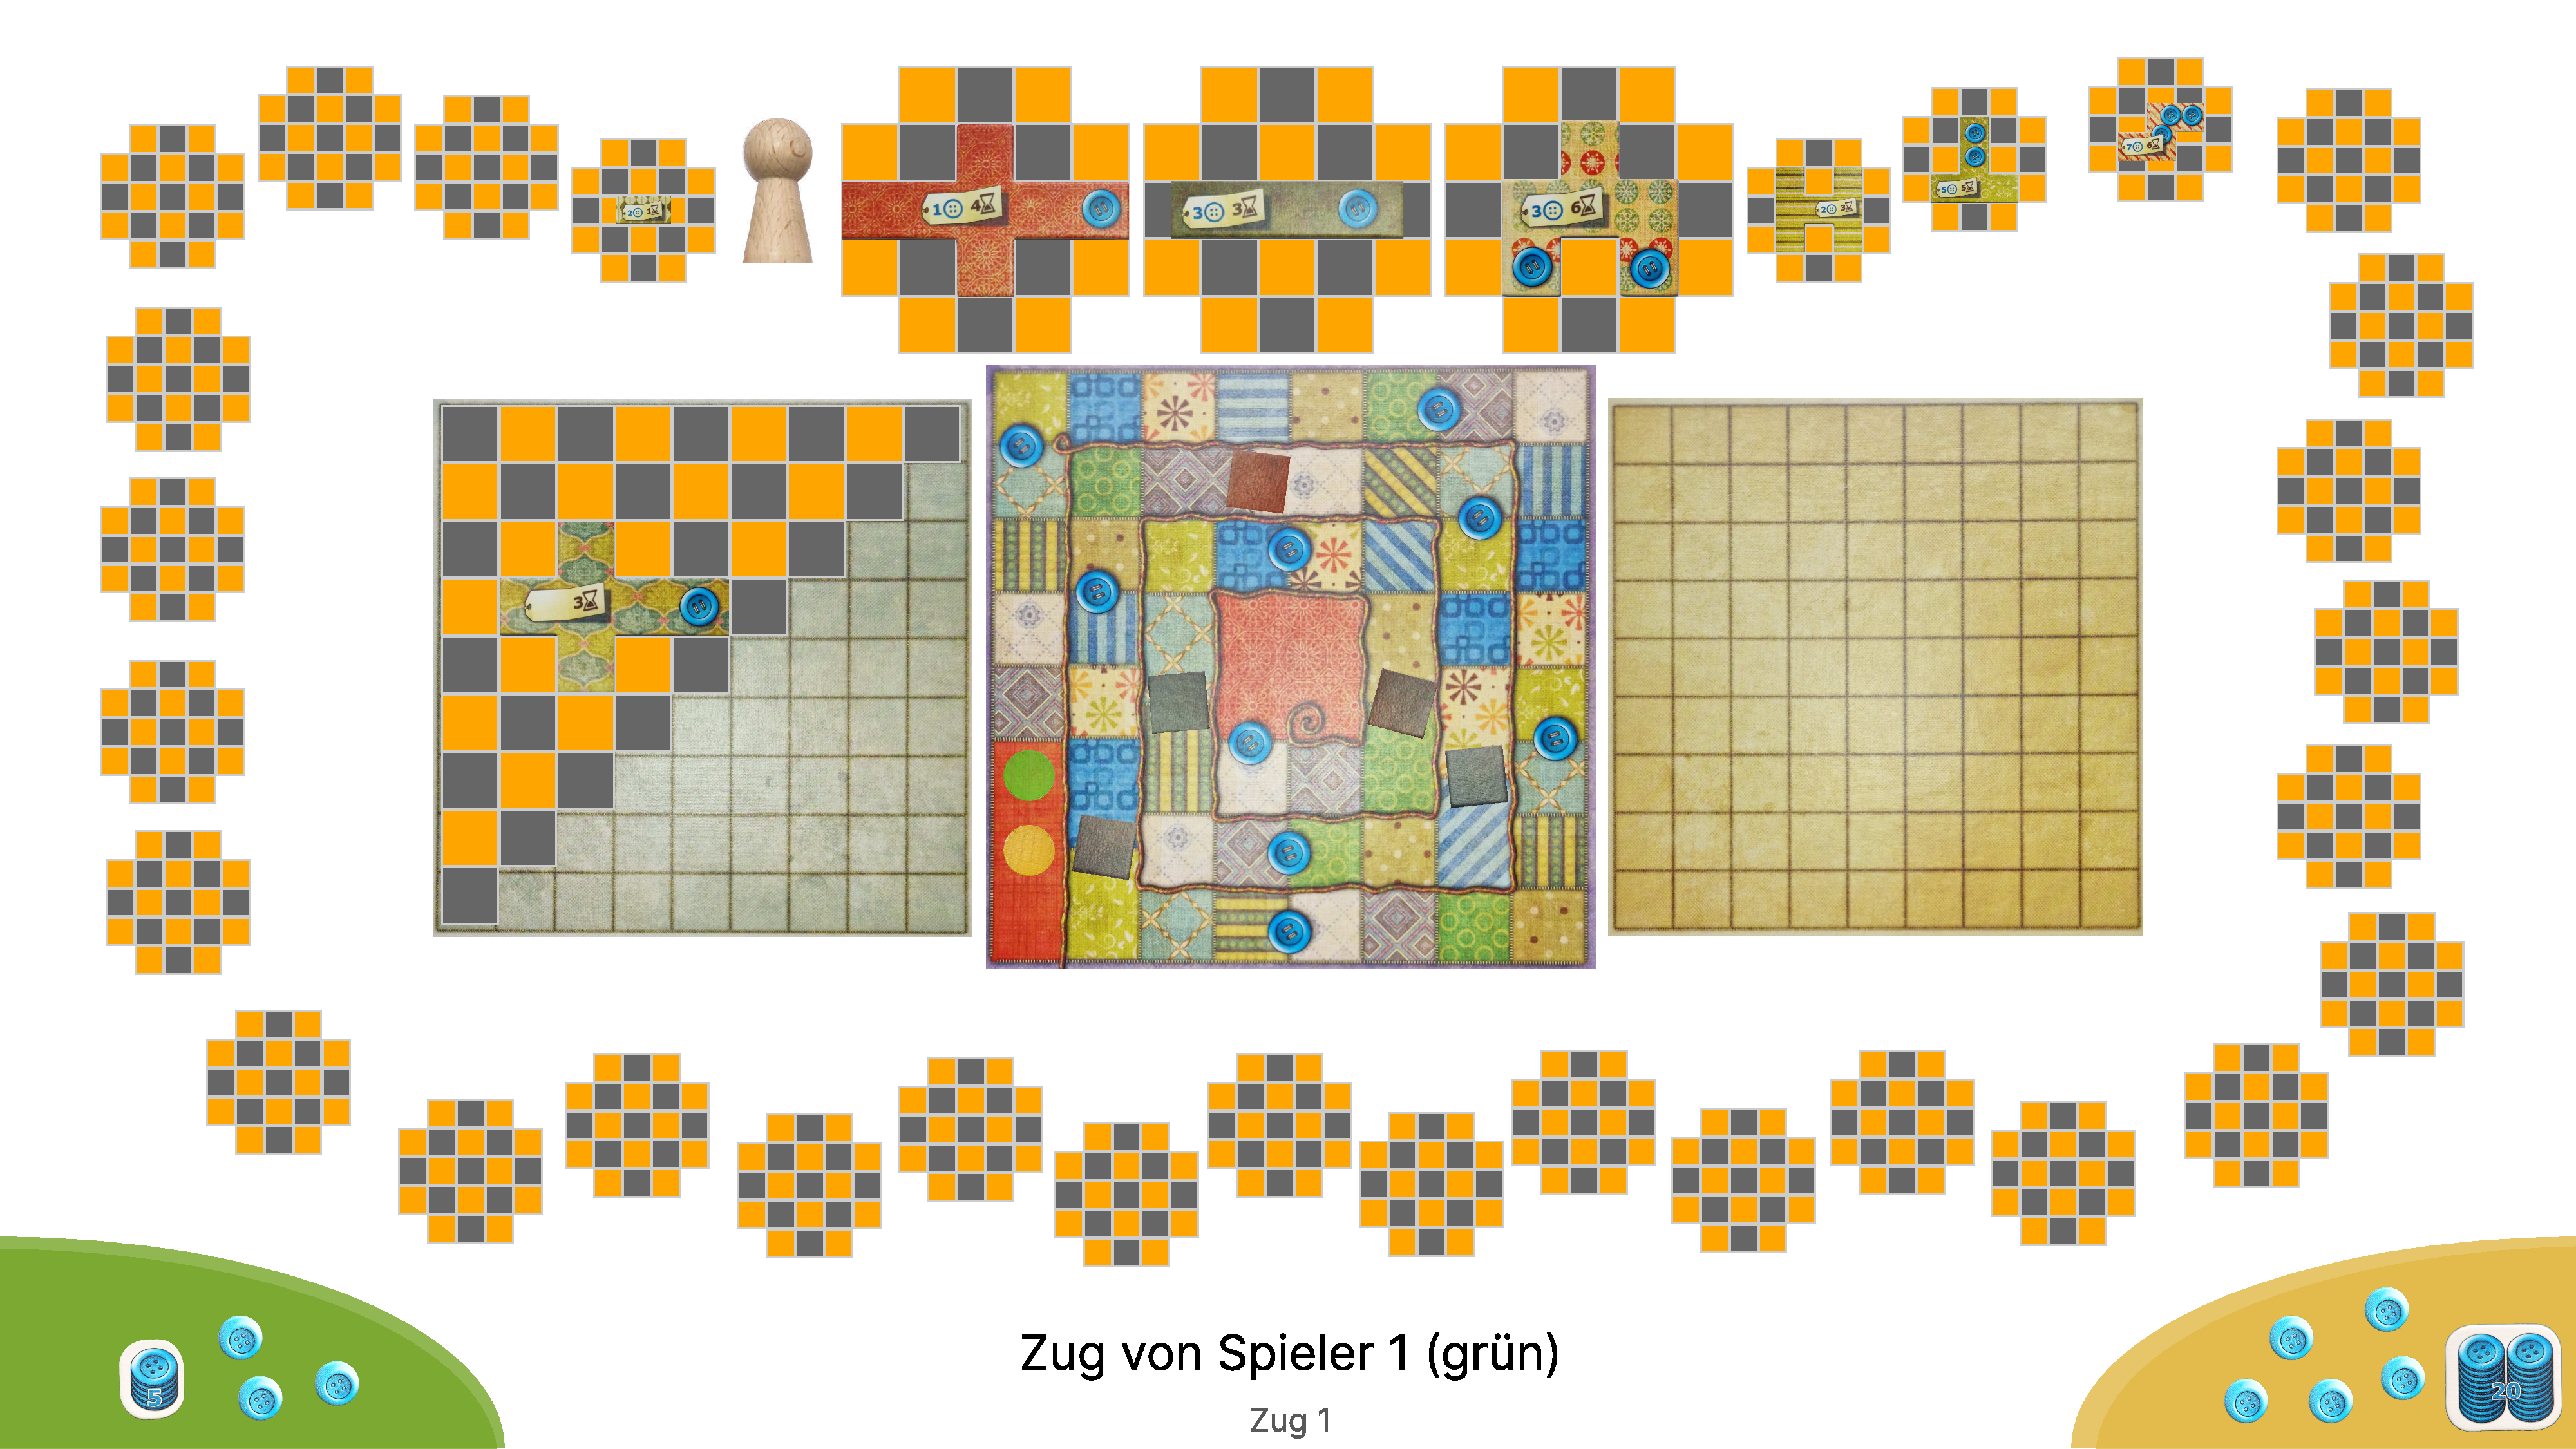
\includegraphics[width=\textwidth]{res/pictures/design_game_ui.pdf}};
        \drawshadow{image}
    \end{tikzpicture}
    \caption{Designentwurf der grafische Benutzeroberfläche des Computerspiel}
    \label{fig:design-game-ui}
\end{figure}